\clearpage

\def\chaptertitle{Introduction}

\lhead{\emph{\chaptertitle}}

\chapter{\chaptertitle}
\label{ch:introduction}

In this chapter, a brief overview of the edge computing architecture paradigm, along with its uses, benefits, and challenges with respect to resource scaling are provided in Section~\ref{sec:ch1-edge-arch}. These challenges lead to the research gap and questions this thesis intends to answer in Section~\ref{sec:ch1-problem-overview}.\par

\section{Edge Computing Overview}
\label{sec:ch1-edge-arch}

Cloud computing architectures leverage the on-demand accessibility of the Internet. The applications deployed here utilize the vast resources of the cloud to perform a task and relinquish it once it is complete for the other sub-modules in the application to request~\cite{rimal2009taxonomy}. In the early days, a singular end-point would be used to access these services, however nowadays the architecture is multi-regional allowing effortless access from across the world. This was achieved through the use of content delivery networks (CDN) located in several regions to allow for data to be quickly replicated and served to clients. This architecture model allows for the processing of large-scale data in a near real-time manner.\par

During the early twenty-first century, this architecture paradigm dominated the Information Technology (IT) industry. Compared to traditional monolithic architectures, the ease of deployment, and scalability, coupled with the economic benefits ensured its dominance. The increasing popularity of hand-held devices as well as home appliances has resulted in data being largely produced at the edge of the cloud network. Thus, processing this large amount of data solely on the cloud proved to be an inefficient solution due to the bandwidth limitations of the network~\cite{shi2016edge}. To counteract this inefficiency, edge computing paradigms were built on the previous foundation of CDNs~\cite{satyanarayanan2017emergence}. Edge computing architectures ensure data processing services and resources exist at the peripheries of the network~\cite{cao2020overview}. The architecture extends and adapts the computing and networking capabilities of the cloud to meet real-time, low latency, and high bandwidth requirements of modern agile businesses.\par

Edge computing deploys several lightweight computing devices known as \textit{cloudlets} to form a ``mini-cloud'' and places them in close proximity to the end-user data~\cite{liu2019survey}. This reduces the latency in terms of client-server communication and data processing. Figure~\ref{fig:edge-architecture-overview} shows a high-level overview of this architecture. Cloudlets can also be easily scaled depending on the resource requirements per edge architecture~\cite{ren2019survey}. However, due to the dynamic resource requirements which may fluctuate from time to time, the resources allocated to cloudlets must be dynamically scaled too. This dynamic scaling, along with the inherent latency present between the cloud layer and the edge cloudlets, poses a significant problem to real-time resource scaling~\cite{varghese2016challenges}.\par

\begin{figure}[htb]
    \centering
    \caption{Overview of edge computing architecture}
    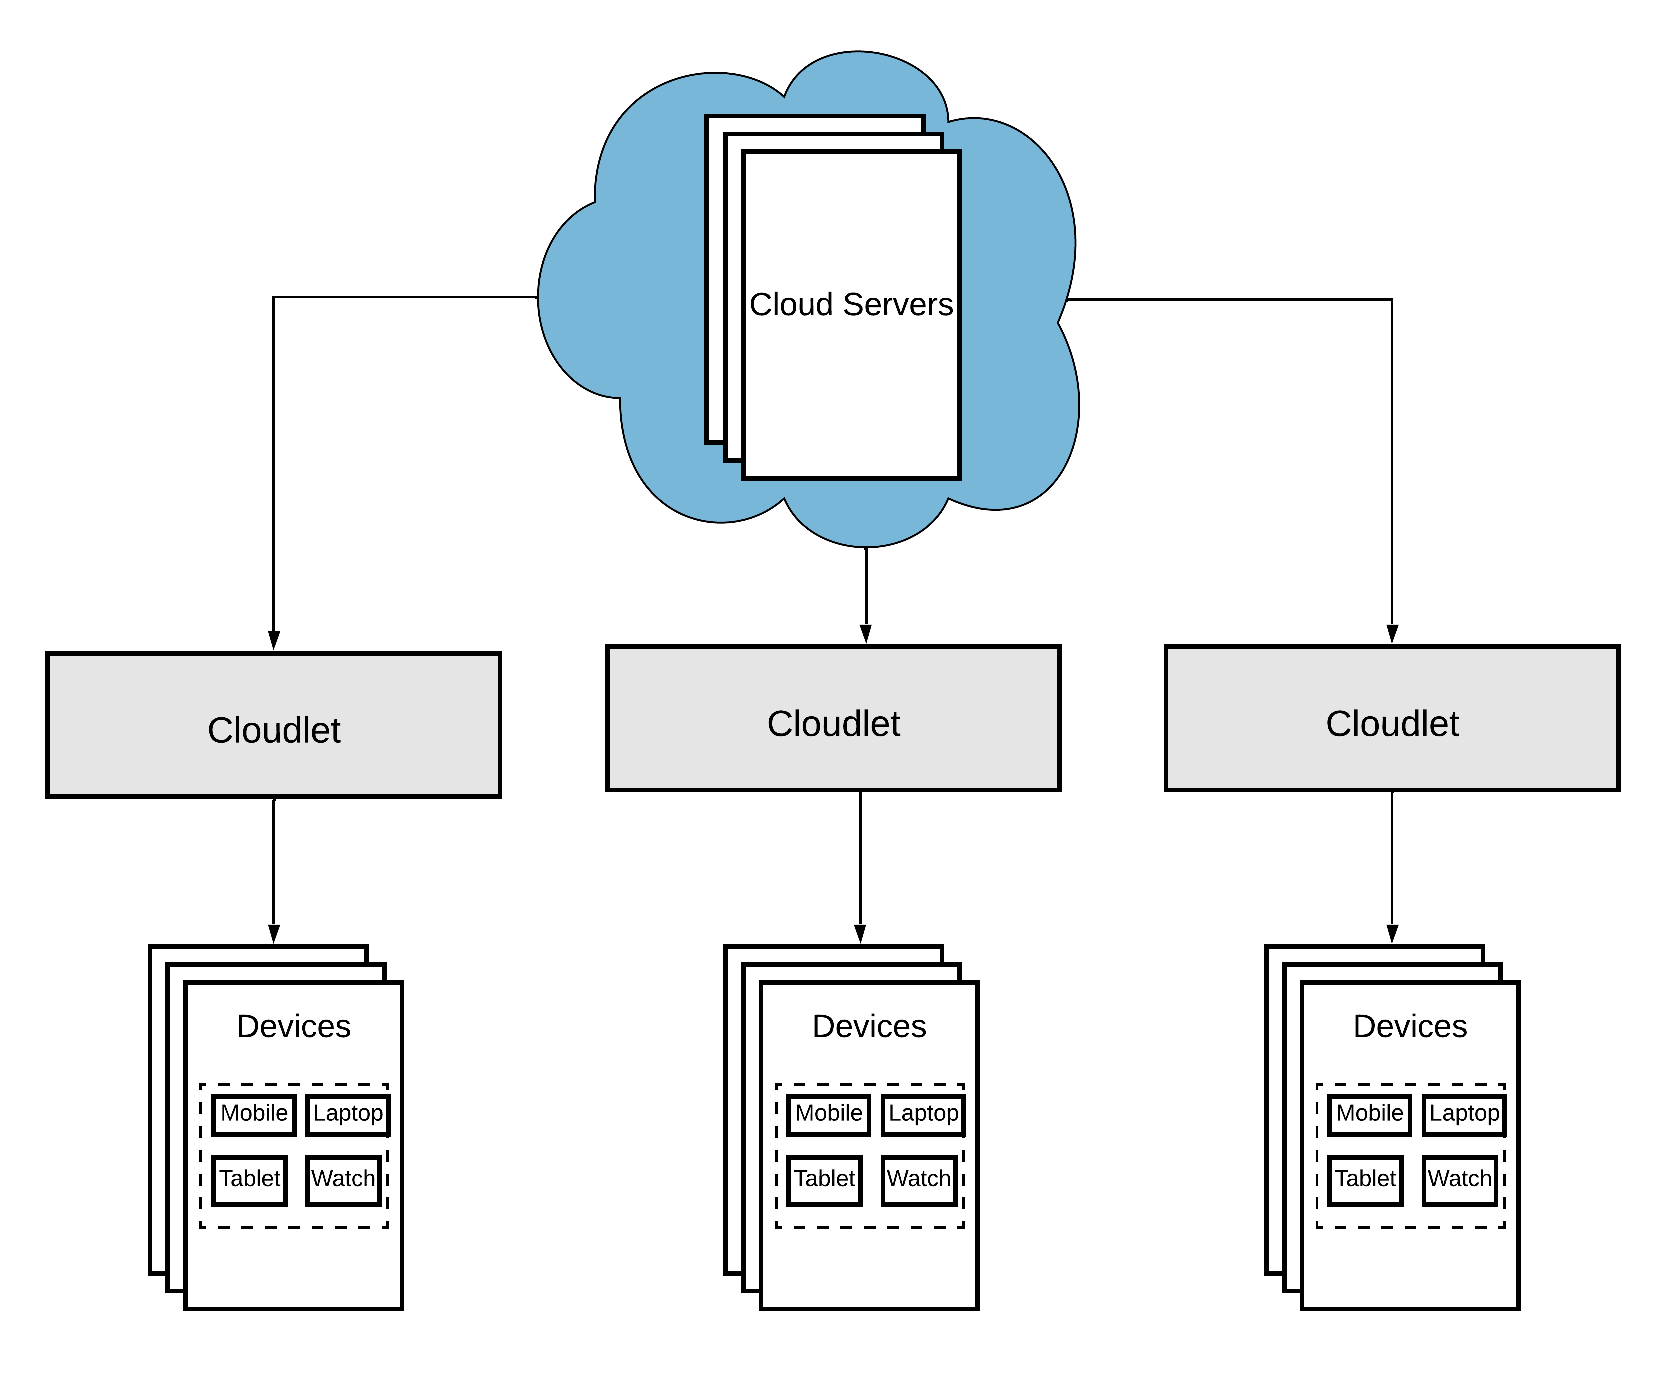
\includegraphics[width=0.9\linewidth]{Figures/Edge-Architecture-Overview.pdf}
    \label{fig:edge-architecture-overview}
\end{figure}

One method of mitigating this scaling latency is through the use of micro-service applications. By employing a micro-service architecture, the resources in a cloudlet are distributed as a collection of smaller deployments that are both independent and loosely coupled~\cite{villamizar2015evaluating}. This loose coupling ensures that parts of the cloudlet can be scaled as required, further reducing the time required to scale resources as compared to scaling the cloudlet monolithically.\par

The scaling of these micro-service resources is done automatically through a process known as auto-scaling. While most container orchestration platforms come bundled with default auto-scaling solutions, and these solutions are sufficient for most applications, they fall apart when scaling resources for time-sensitive services processing real-time data such as the ones used in healthcare require stringent compliance to service level agreements (SLA) on metrics such as application latency. This has led to further research on auto-scaling solutions for edge computing applications. These primarily fall into two categories. Reactive auto-scaling solutions attempt to modify the micro-service resource allocation once the required resources exceed the current allocation. These algorithms are simple to develop and deploy, however, the time taken to scale resources leads to a degradation of resource availability and violates SLA compliance~\cite{podolskiy2018iaas}. To counteract these pitfalls, proactive auto-scaling solutions attempt to model resource allocation over time and effectively predict the resource requirements. By doing so, the micro-service resources can be scaled in advance through a process known as ``cold starting''. This approach removes the latency inherent in scaling resources, however, the algorithms are extremely complex to develop, train, and tune to specific edge applications~\cite{straesser2022not}.

\section{Objectives and Thesis Structure}
\label{sec:ch1-problem-overview}

To tackle these challenges, this thesis proposes a hybrid approach that combines the simplicity of using reactive autoscalers, while maintaining the resource availability benefits of the proactive autoscalers. The algorithm involves a smaller-scale LSTM machine learning model which can be quickly trained to recognize the key features of the resource workload over a course of time. The autoscaler then uses the predictions from the LSTM model to scale its resources in advance. A reactive autoscaler is used to maintain the current resource requirements as the predictive model cannot provide fine-tuned predictions. The accuracy of the prediction model is gauged by monitoring the SLA metrics, for example, the application latency. If it is observed that the predictive model is performing poorly, the training parameters are automatically tuned for the next training iteration.\par

Thus, this project aims to answer the following research questions:

\begin{itemize}
    \item \textbf{\textit{RQ1:}} Can we integrate reactive and proactive auto-scaling methods to develop a tailored algorithm for edge computing that eliminates the requirement to fine-tune hyper-parameters for each auto-scaling use case while being lightweight enough to be deployed and run on cloudlets?
    \item \textbf{\textit{RQ2:}} Can the hybrid auto-scaling solution achieve or exceed the SLA compliance capabilities of state-of-the-art reactive and proactive auto-scaling solutions for edge computing while minimizing the cost of deploying application resources?
\end{itemize}

The thesis structure was designed based on the general guidelines provided by Gruba and Zobel~\cite{gruba2017write}. In summary, the following contributions were made in this thesis:

\begin{itemize}
    \item Propose a hybrid auto-scaling method that mitigates the challenges present in reactive and proactive methods.
    \item The algorithm is implemented as an extension to Kubernetes.
    \item Deploy this algorithm in a real edge cluster prototype.
    \item Conduct extensive experiments using realistic daily workloads on the prototype micro-service application.
    \item Compare the SLA violations of the cutting-edge reactive, proactive, and default container orchestration autoscaler with the proposed hybrid algorithm for three separate threshold categories.
    \item Propose future work and possible extensions to the algorithm.
\end{itemize}
